\documentclass[a4paper, 10pt]{article}
\usepackage[margin = 1in]{geometry}
\usepackage{amsmath}
\usepackage{tabularx}
\usepackage{framed}
\setlength{\parindent}{0em}
\newcolumntype{L}{>{\arraybackslash}m{10cm}}
\newcolumntype{T}{>{\arraybackslash}m{6cm}}
\usepackage{graphicx}
\usepackage{pdfpages}

\begin{document}

\section*{Topic 19 - Quantum Physics}

\section{Photoelectric effect}

\begin{framed}
   The \textbf{photoelectric effect} is a process in which electrons are emitted from a metal surface when an electromagnetic radiation of sufficiently high freqeuency is incident on the surface \\
   A \textbf{photoelectron} is an eelctron emitted from the surface of a material due to the incident electromagnetic radiation
\end{framed}	

\subsection{The photoelectric experiment}
\begin{center}
   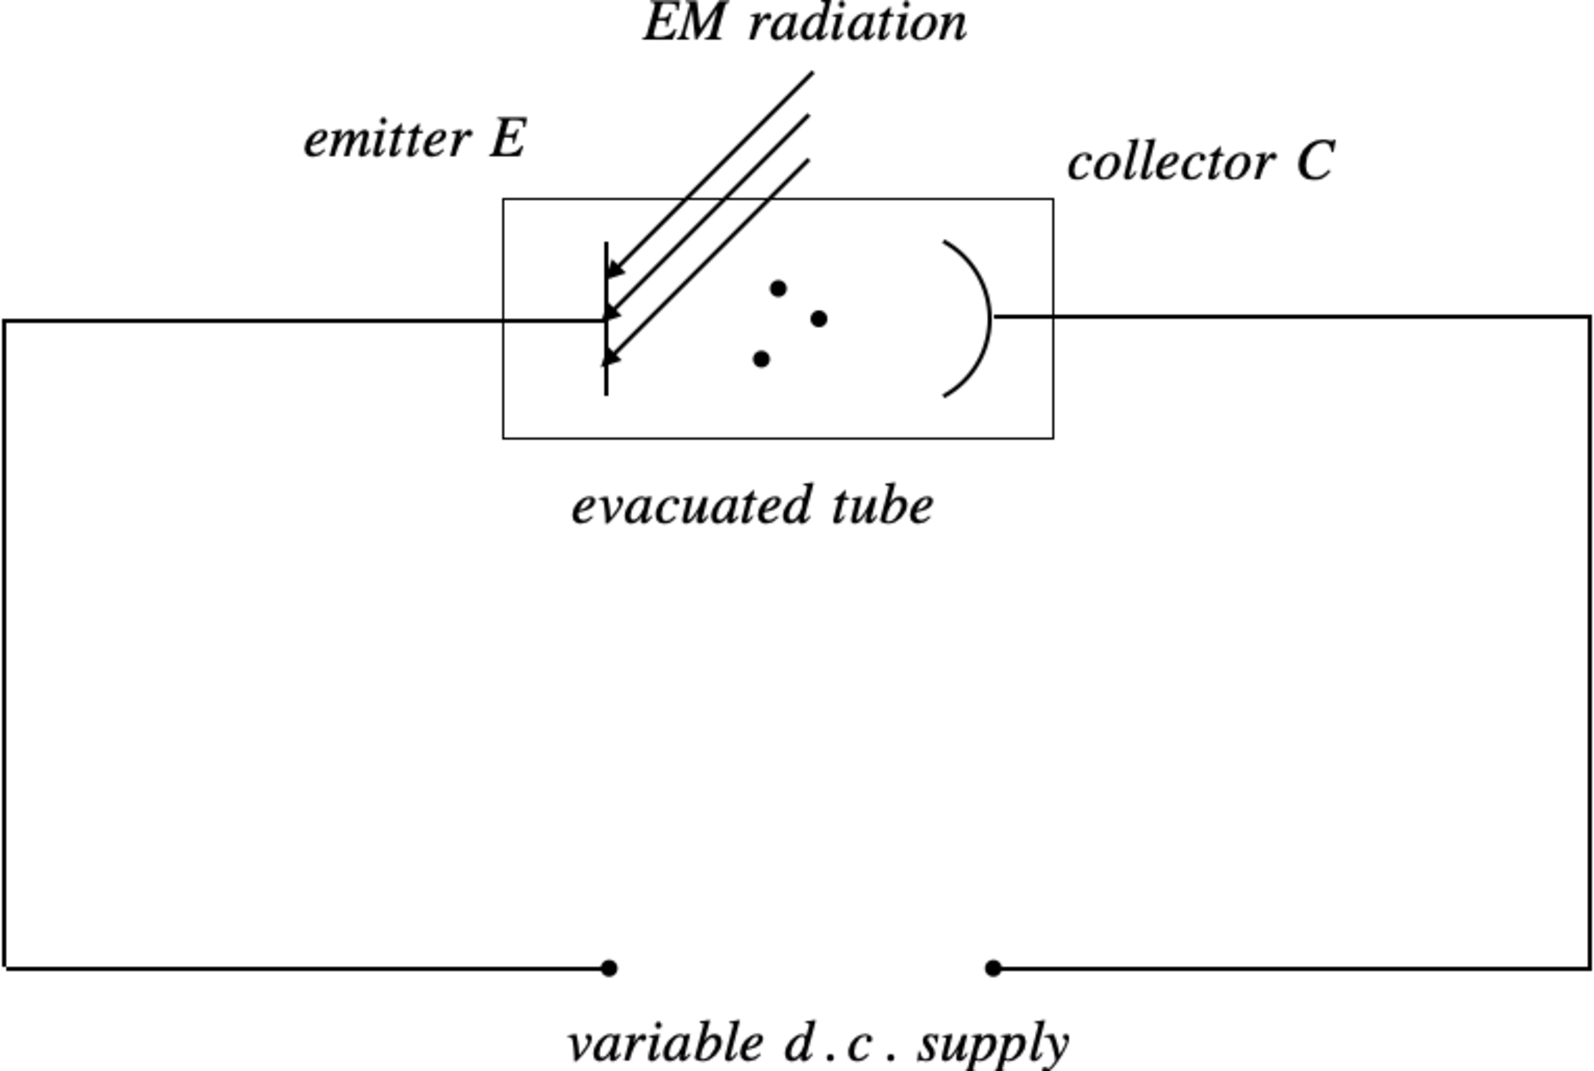
\includegraphics[width=3in]{figures/1.pdf} 
\end{center}

\begin{center}
   \begin{tabular}{T | T}
      when collector C is sufficiently positive wrt E & when collector C is sufficiently negative wrt E \\
      \[
         V_{CE} = +ve 
      \] &
      \[
         V_{CE} = -ve
      \] \\
      \begin{itemize}
         \item all photoelectrons attracted to C
         \item rate of emission of photoelectrons = rate of electrons reaching C
         \item ammeter reads constant \textbf{saturated photocurrent, $i_0$ }
            \[
               \text{rate of emission of $e^-$ } = \frac{dN_e}{dt} = \frac{i_0}{e}
            \]
      \end{itemize}	  &
      \begin{itemize}
         \item most energetic photoelectrons do not have sufficient energy to reach C
         \item photocurernt $i$ is zero
            \[
               KE_{max} = eV_s
            \]
      \end{itemize}	
   \end{tabular}
\end{center}

\subsection{Stopping potential $V_s$ }
\begin{framed}
   \textbf{Stopping potential} is the negative potential of colelctor wrt emitter which prevents the most energetic photoelectrons from reaching the collector and hence resulting in \textbf{zero photocurrent}
\end{framed}	

\subsection{Discrepencies with classical wave theory}
      By classical wave theory, the intensity of a wave is defined as the energy incident per unit area per unit time
      \[
      I = \frac{E}{tA}
      \]
\begin{enumerate}
   \item Absence of time lag \\

      By classical wave theory, electrons should absorb energy over a period of time before it gains enough energy. 

   \item Existence of threshold frequency \\

      Since Energy of a wave is dependednt on the square of its amplitude, photoelectrons should be emitted if radiation of sufficient intensity is used, and no threshold frequency should be observed
   \item Max K.E. is independent of intensity but varies with frequency\\

      By classical wave theory, the stopping potential $V_s$ should increase with intensity of light, since light of higher intensity should eject photoelectrons with greater KE.
\end{enumerate}	

\subsection{Quantum theory of light}

\begin{framed}
   Light and other forms of EM radiation are emitted in discrete packets of energy called 'quantum', and the energy $E$ in each quantum emitted is given by
   \[
   E = hf
   \]
   where $h = 6.63 \times 10^{-34}Js $ \\
  
   A \textbf{photon} is a quantum of electromagnetic energy.  \\

   By substituting $c = f\lambda$, the energy of a photon is
   \[
    E = hf = f \frac{c}{\lambda}
   \]
   where $c = 3.00 \times 10^8 ms^{-1}$ 
\end{framed}	

Hence a monochromatic beam of light containing $N$ photons has total energy
\[
   E_{total} = Nhf = Nh \frac{c}{\lambda}
\]

in relation to the photoelectric experiment, 
\begin{itemize}
   \item a stream of photons bombard surface of metal
   \item free electrons near the surface could be struck by a photon and gains the \textbf{whole amount of energy}. 
   \item if the gain in energy is sufficient, the electorns can leave the plate as a photoelectron
   \item the energy of a photon must be completely absorbed by a \textbf{single electron}, otherwise it is reflected or transmitted. 
\end{itemize}	

\subsection{Einstein's photoelectric equation}
\begin{framed}
   the \textbf{work function energy $\Phi$} of a metal is defined as the \textbf{minimum amount of energy} necessary for an electron to escape from the surface of a metal
\end{framed}	

\begin{framed}
   \textbf{Einstein's photoelectric equation} states that the 
   \[
      \text{photon energy} = \text{work function energy} + \text{maximum KE of photoelectron}
   \]
   \[
      hf = \Phi + \frac{1}{2} m_e v_{max}^2
   \]
\end{framed}	

\subsection{Einstein's photoelectric equation applied to the photoelectric experiment}
\begin{enumerate}
   \item Max KE independent of intensity and varies linearly with frequency \\

      Photoelectrons with max KE come from surface of the metal. Those below the surface lose energy due to collision with atoms and are emitted with \textbf{lower KE} \\

      KE varies up to a maximum given by
      \[
         KE_{max} = hf - \Phi
      \]
   \item Existance of threshold frequency $f_0$ \\

     When KE is zero, no electrons can escape
     \[
     \Phi = hf_0
     \]

     Hence KE is only greater than zero for $f > f_0$ 
     \begin{framed}
        \textbf{Threshold frequency} is the minimum frequency of EM radiation below which no emission of photoelectrons occur
     \end{framed}	


  \item Absence of time lag \\

     photoelectrons are emitted immediately after gaining energy from a photon. All of a photon's energy is transferred immediately upon collision. Hence emission has no time lag
      
\end{enumerate}	

\subsection{Photoelectric equation applied to stopping potential $V_s$}

For the most energetic photoelectrons
\[
   \text{decrease in KE} = \text{increase in EPE}
\]

\[
   \frac{1}{2}m_e v_{max}^2 - 0 = eV_s
\]
\[
   KE_{max} = eV_s
\]

Rewriting Einstein's photoelectric equation
\[
   KE_{max} = hf - \Phi
\]
\[
eV_s = hf - \Phi = hf - hf_0
\]
\[
   V_s = \frac{h}{e}f - \frac{\Phi}{e}
\]

\subsection{Associated graphical representations of photoelectric results}
\subsubsection{intensity - current graphs}
\begin{minipage}{0.5\textwidth}
   \begin{center}
    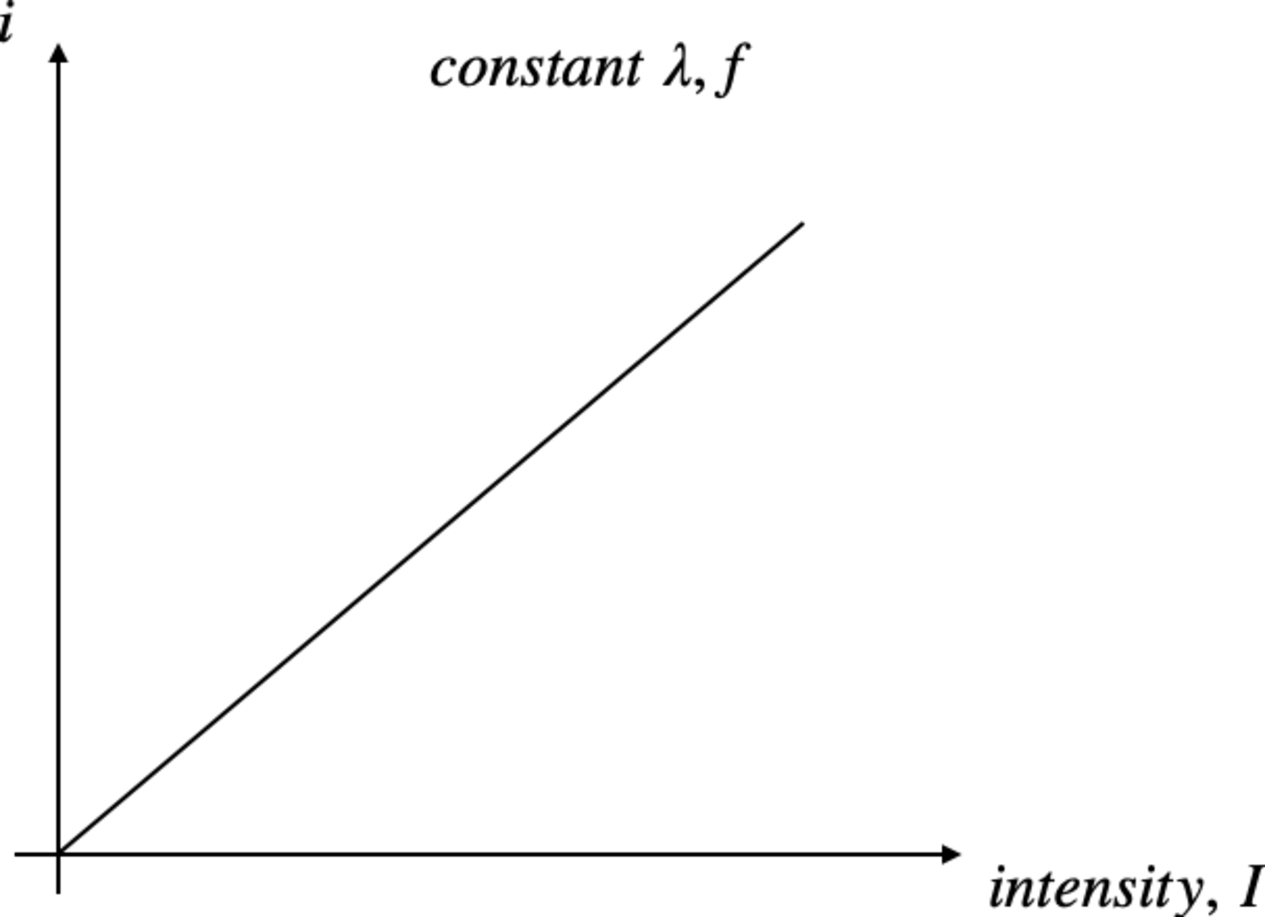
\includegraphics[width=3in]{figures/2.pdf} 
   \end{center}	
\end{minipage}
\begin{minipage}{0.5\textwidth}
   \[
   \frac{dN_e}{dt} \propto \frac{dN_p}{dt}
   \]
   \[
   intensity = \frac{P}{A} = \frac{E}{tA} = nhf
   \]
   \[
   I \propto \frac{dN_p}{dt} \propto \frac{dN_e}{dt}
   \]
\end{minipage}

\subsubsection{Stopping potential - frequency graphs}
\begin{minipage}{0.5\textwidth}
\begin{center}
   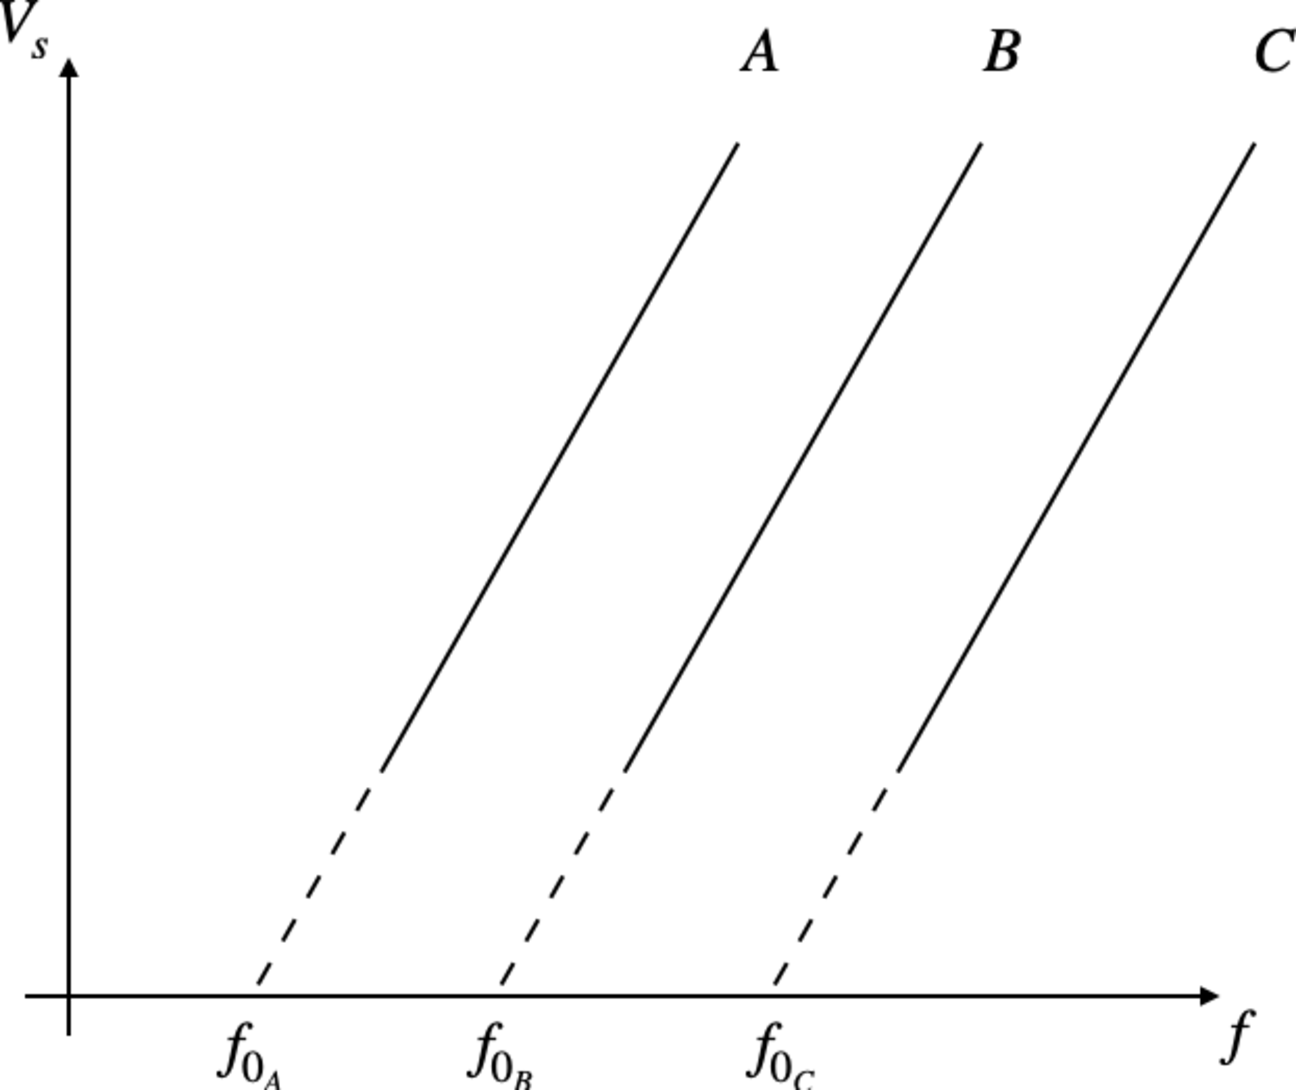
\includegraphics[width=5cm]{figures/3.pdf} 
\end{center}	
\end{minipage}
\begin{minipage}{0.5\textwidth}
  \[
     V_s = \frac{h}{e} f - \frac{\Phi}{e}
  \]

  A similar graph of $KE_{max}$ against $f$ could be obtained
\end{minipage}

\subsection{Potential difference - current graphs}
\begin{minipage}{0.5\textwidth}
   \begin{center}
      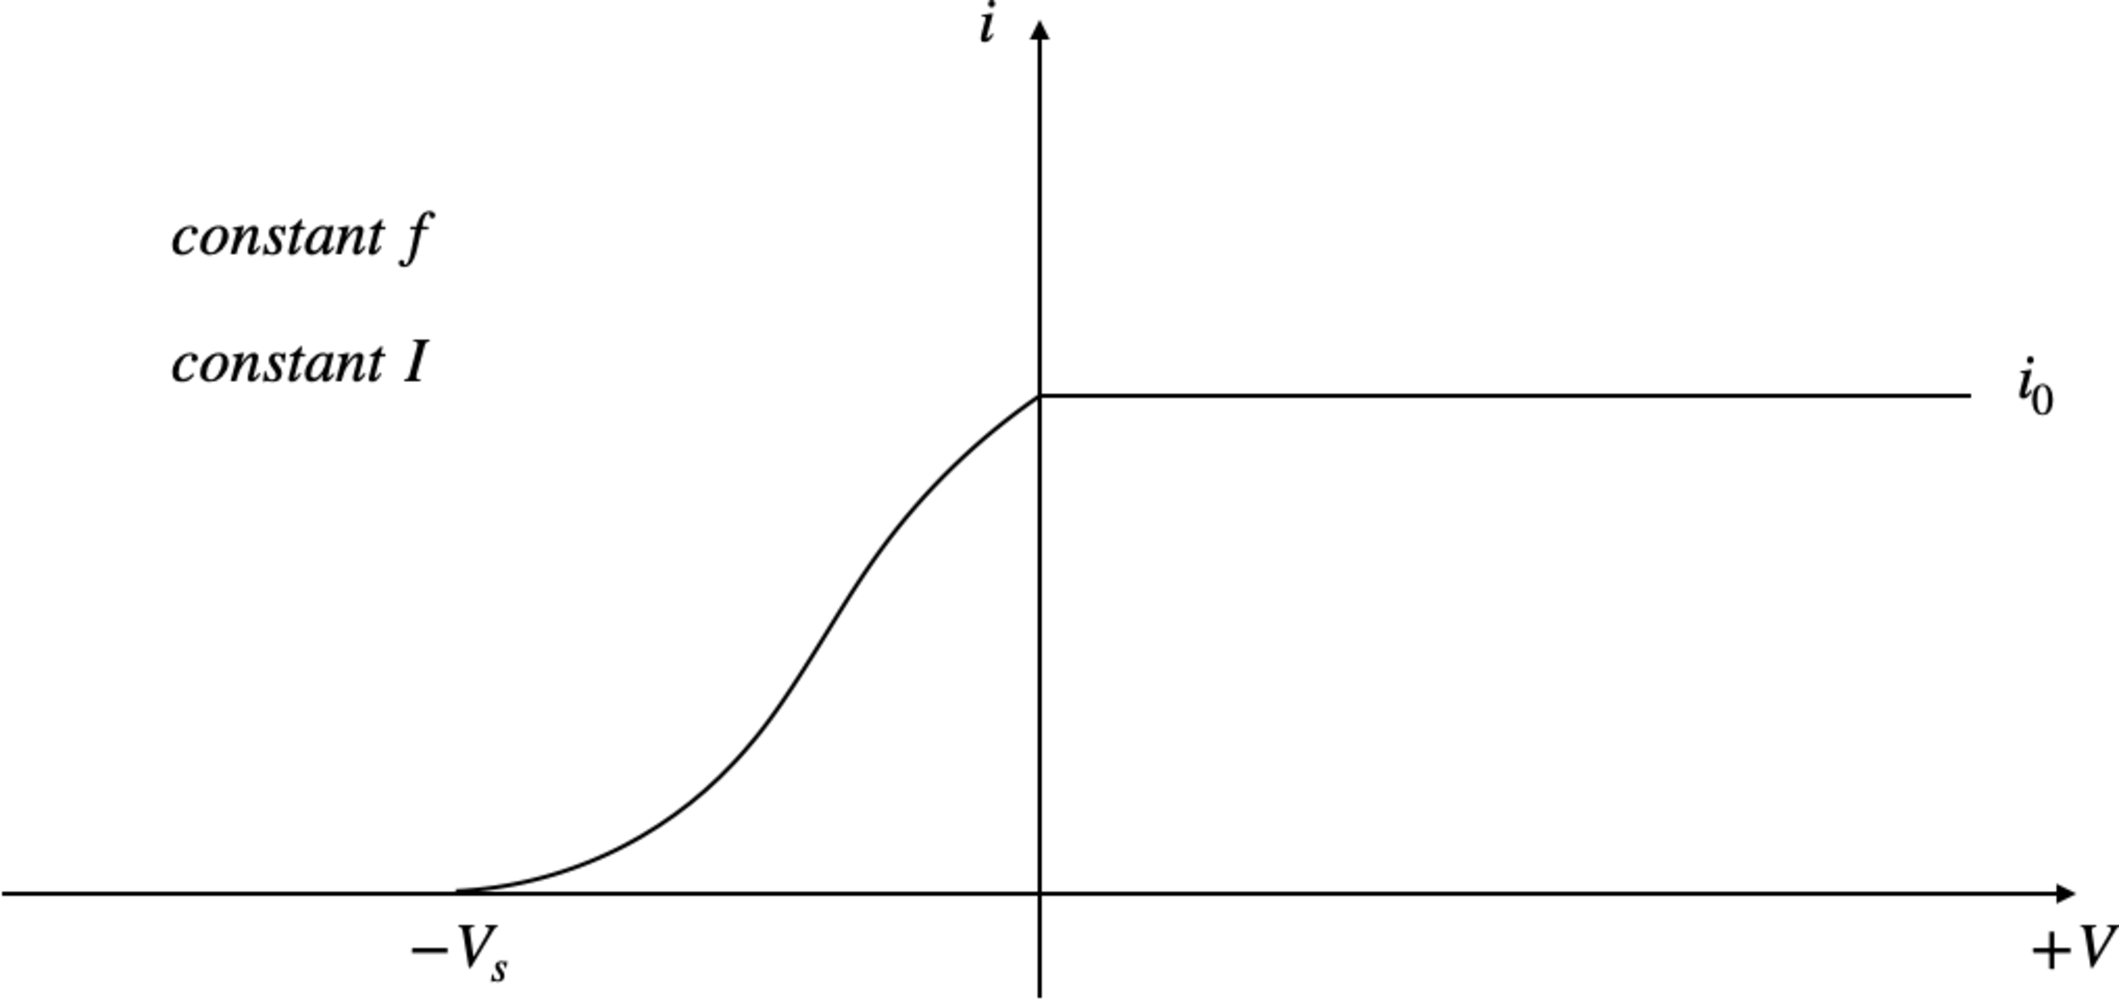
\includegraphics[width=3in]{figures/4.pdf} 
   \end{center}	
\end{minipage}
\begin{minipage}{0.5\textwidth}
   \begin{itemize}
      \item when $V_{CE}$  is positive, all emitted electrons reach collector, hence \textbf{photcurrent, $i$ is at maximum, $i_0$ }
      \item As $V_{CE}$ becomes more negative, more electrons are repelled from collector, hence $i$ decreases
      \item $i$  reaches 0 when $V_{CE} = V_s$, and \textbf{not even the most energetic photoelectrons} can reach collector. stopping potential is given by
         \[
            eV_s = KE_{max}
         \]
   \end{itemize}	
\end{minipage}


\begin{minipage}{0.5\textwidth}
   \begin{center}
      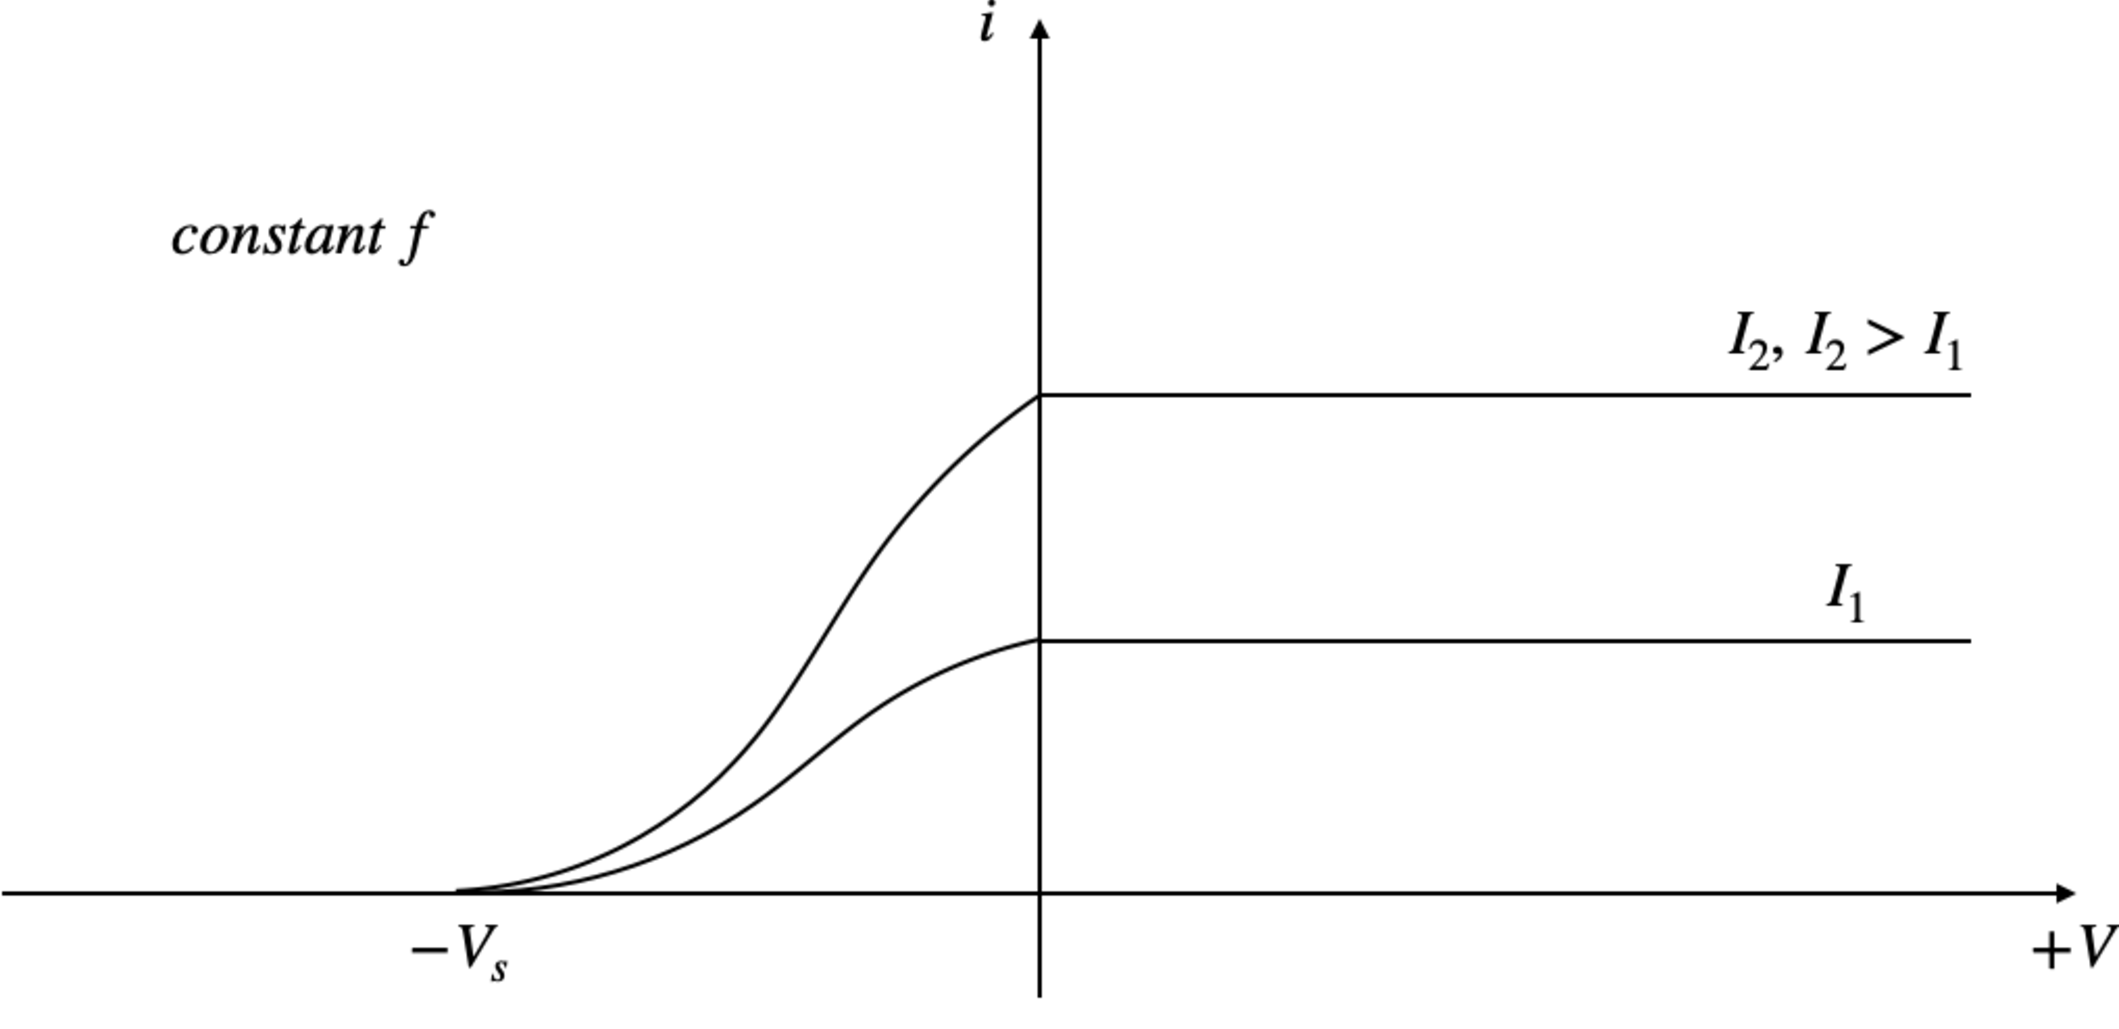
\includegraphics[width=3in]{figures/5.pdf} 
   \end{center}	
\end{minipage}
\begin{minipage}{0.5\textwidth}
   \[
   i_0 \propto I
   \]
   Since 
   \[
      KE_{max} = eV_s = hf - \Phi
   \]
   $V_s$ constant
\end{minipage}



\begin{minipage}{0.5\textwidth}
   \begin{center}
      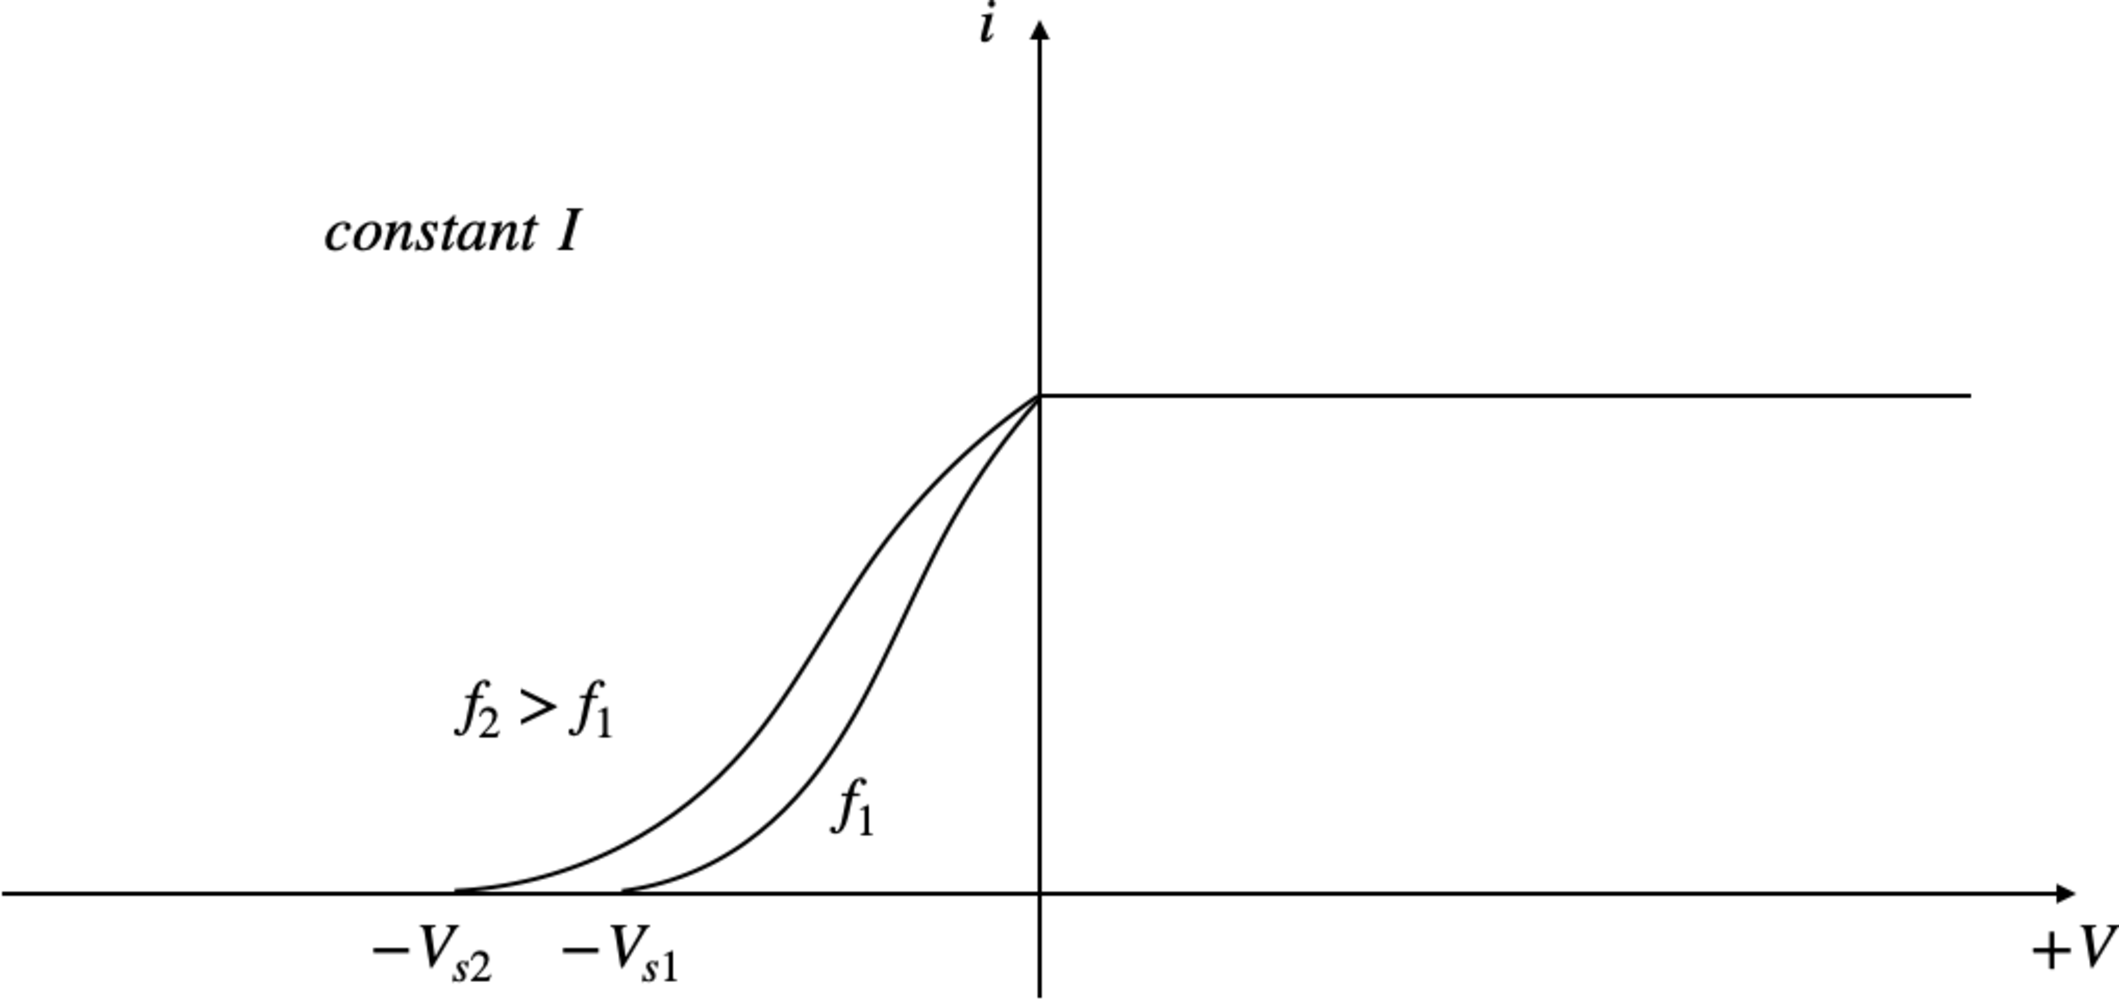
\includegraphics[width=3in]{figures/6.pdf} 
   \end{center}	
\end{minipage}
\begin{minipage}{0.5\textwidth}
   \[
   V_s \propto f
   \]
   
\end{minipage}

\section{Wave-particle duality}

\begin{framed}
   \textbf{The theory of wave-particle duality} states that matter and waves have particle-like and wave-like properties

   The \textbf{De Broglie wavelength} is the wavelength associated with wave-like properties of a particle
\end{framed}	

\begin{framed}
   For a particle with momentum \textbf{p = mv}, the associated De Broglie wavelength is 
   \[
     \lambda = \frac{h}{p} = \frac{h}{mv}
   \]
   
   For EM radiation with wavelength $\lambda$, the radiation exhibits particle behaviour with associated momentum 
   \[
   p = \frac{h}{\lambda} = \frac{hf}{c}
   \]
   
\end{framed}	

\begin{center}
   \begin{tabular}{c | c | c}
      & Evidence for wave-like properties & Evidence for particle-like properties \\ \hline
      Light & Interference, diffraction & Photoelectric effect, emission spectra \\ \hline
      Electrons & Diffraction & Electrons have mass and charge, and undergo collision 
   \end{tabular}
\end{center}

\section{Energy levels and line spectra}

\subsection{Quantisation of energy levels and Bohr's atomic model}

\begin{minipage}{0.5\textwidth}
   \begin{center}
      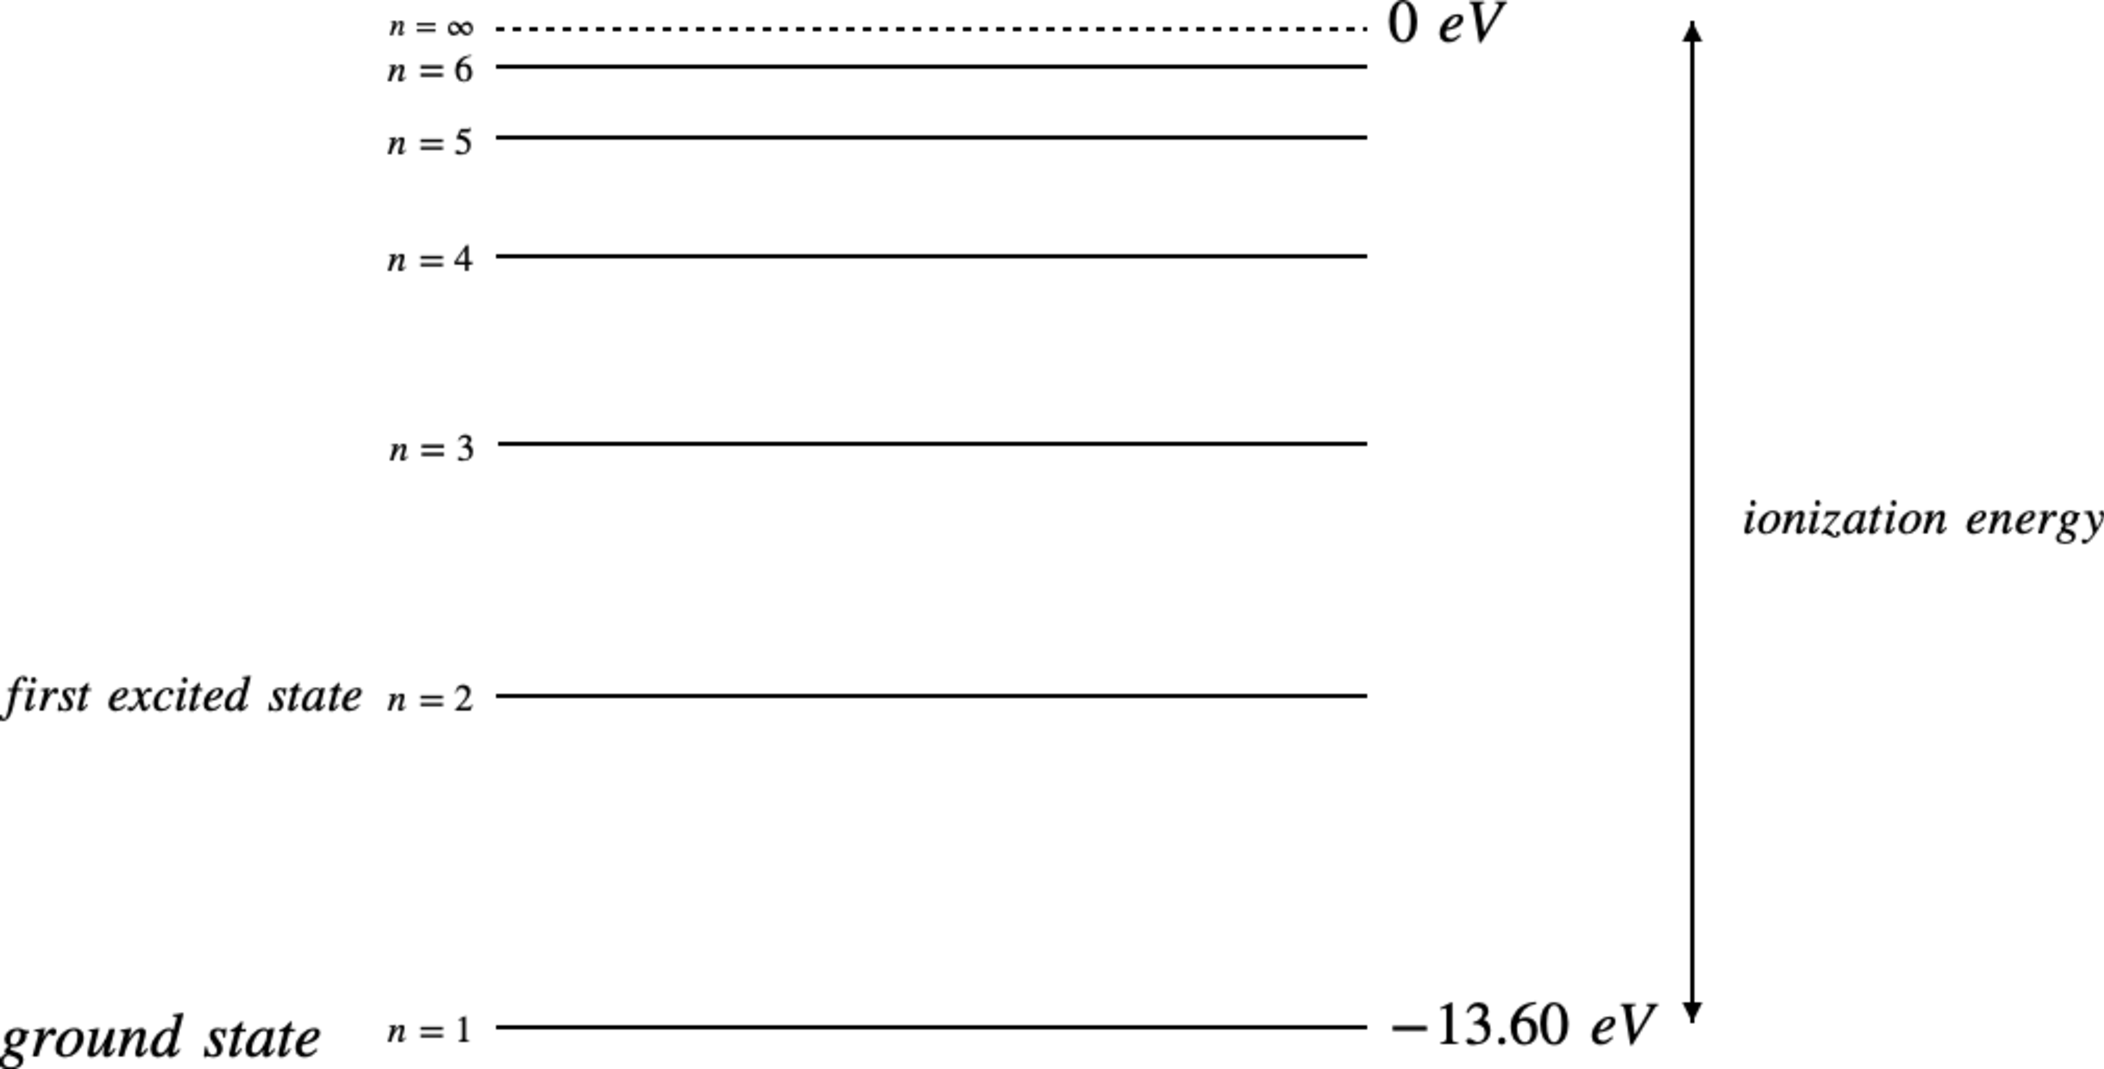
\includegraphics[width=3in]{figures/7.pdf} 
   \end{center}	
\end{minipage}
\begin{minipage}{0.5\textwidth}
   Bohr postulated that
   \begin{itemize}
      \item There are only certain allowed orbits in the atom
      \item Electrons are in stable state or \textbf{ground state} when they occupy orbits corresponding to \textbf{lowest} energy levels
      \item An atom radiates energy when elcetron transits from a more energetic state to a lower energy state. The energy is emitted as \textbf{one quantum} 
         \[
         E_i - E_f = hf
         \]
         
   \end{itemize}	
\end{minipage}

\subsection{Excitation and de-excitation of atomss}

\textbf{Ionisation} is the process of creating charged particles \\

\textbf{Excitation} is the process where atoms absorb energy without ionisation. Excitation occurs due to 
\begin{enumerate}
   \item \textbf{Particle collision }\\

      A high speed particle collides and imparts its energy to an electron. It can transfer \textbf{part or whole} of its energy. \\

      Energy transferred must be sufficient for electron to \textbf{transit to higher energy level} but \textbf{needs not match} the difference in energy  levels

   \item \textbf{Photons} \\

      If a photon with energy \textbf{exactly equal} to the energy difference between 2 levels in the atom collides with an orbital electron, the photon will be absorbed.  \\

      If photon's energy is not exactly equal, it will not be absorbed
\end{enumerate}	

During \textbf{De-excitement}, excited orbital electrons return to a lower energy state and give off excess energy in the form of photons


\subsection{Emission line spectrum}
\begin{center}
   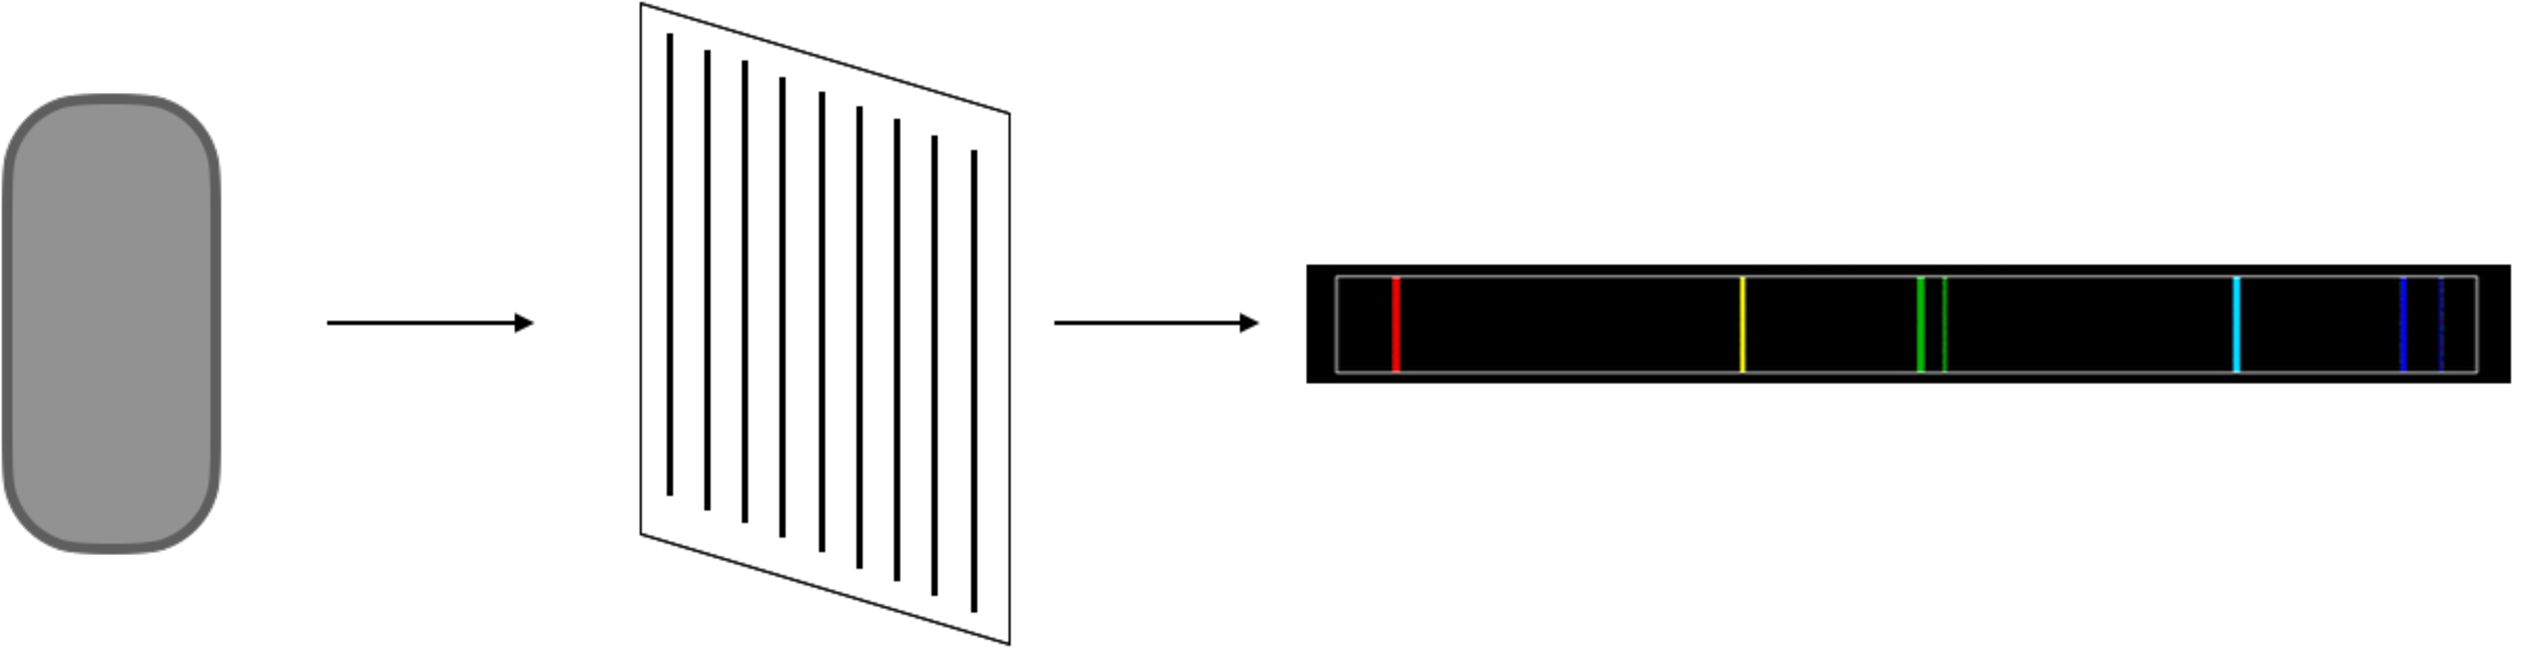
\includegraphics[width=3in]{figures/8.pdf} 
\end{center}	
\begin{itemize}
   \item A gas is placed in a discharge tube at \textbf{low pressure} and \textbf{high voltage}
   \item When gas is heated / bombarded with electrons, the electrons in gas atoms are excited to higher energy levels
   \item The excited electrons remain in higher energy state momentarily before de-exciting to lower energy.
   \item Upon de-exciting, photons are emitted with energy  corresponding to the energy difference
   \item The gas starts to glow and light is emitted from discharge tube
   \item When light is exxamined through diffraction grating or spectrometer, a spectrum of distinct, well-defined lines is observed.
\end{itemize}	

\subsection{Absorption line spectrum}

\begin{itemize}
   \item When white light containing all visible frequencies passes through a \textbf{cool gass}, the atoms of cool gas absorb photons of certain frequencies to jump to a higher energy level. 
   \item After excitation, the atoms eventually return to lower energy state by emitting the same photon it absorbed. 
   \item
\end{itemize}	













\section{X-ray spectrum}
\section{Heisenberg uncertainty principle}

\end{document}	
